\afterpage{
     \begin{figure}[t!]
         \centering
         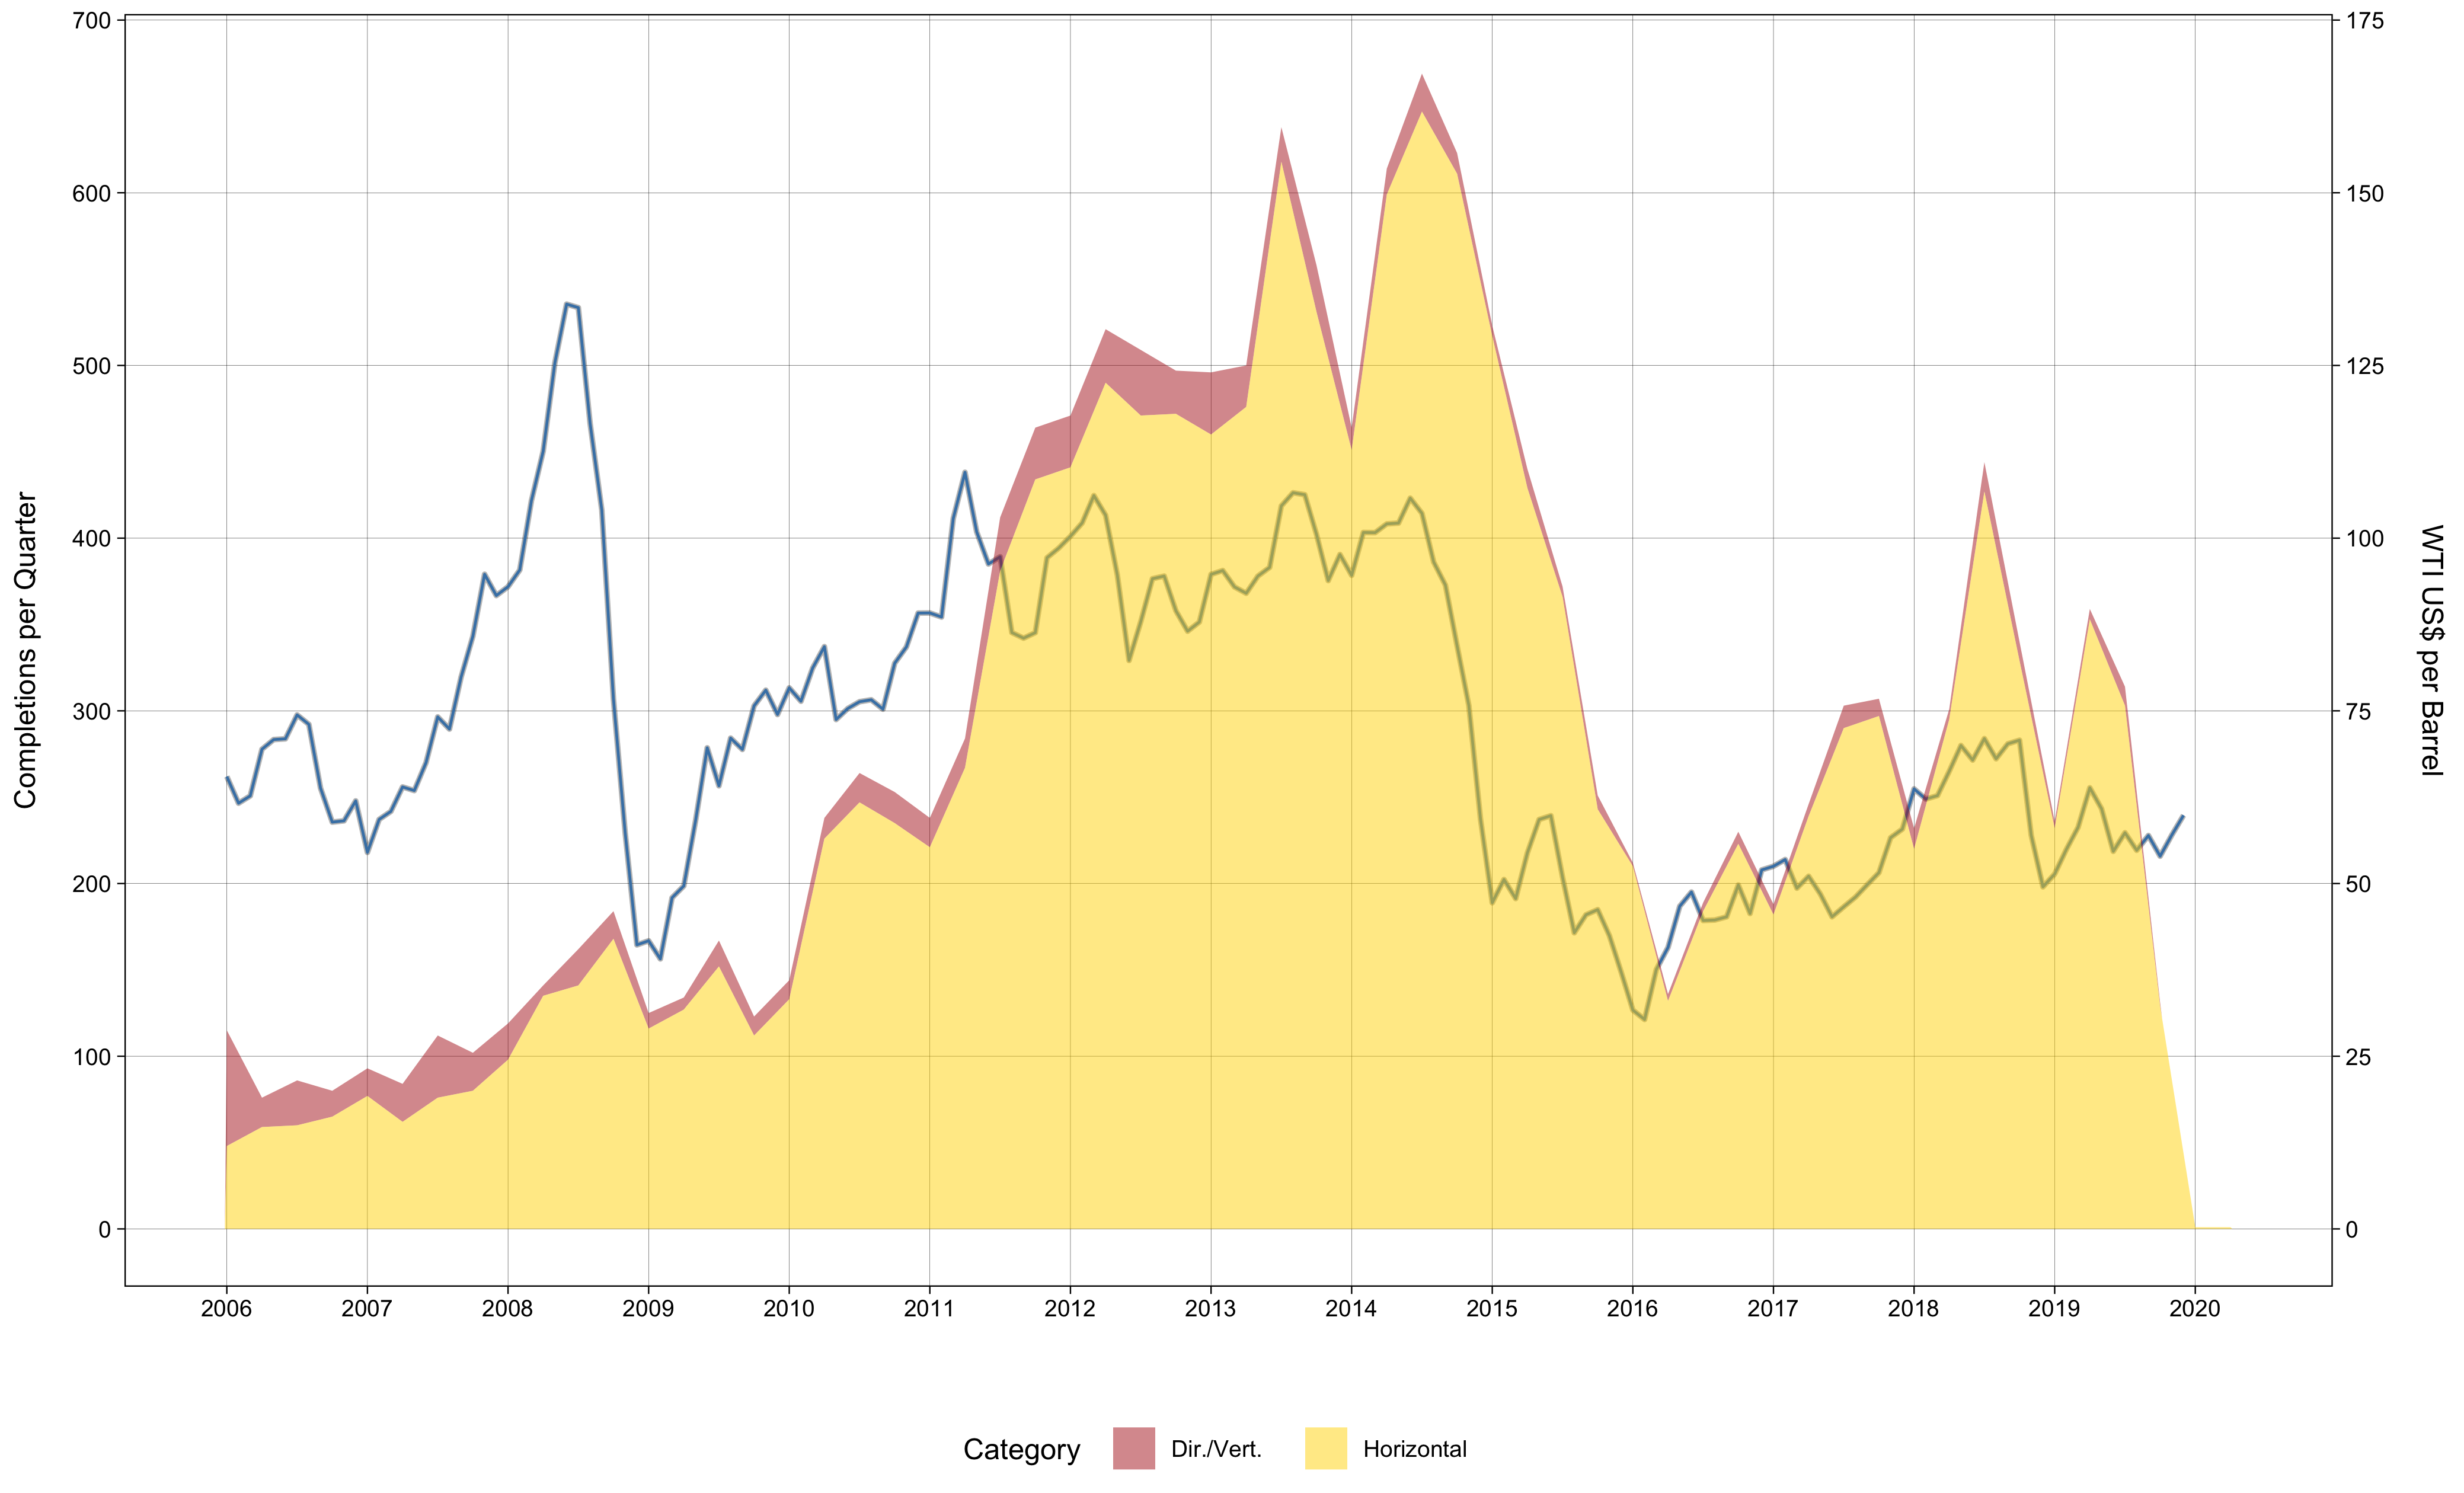
\includegraphics[scale = 0.105]{04_Chapter-3/00A_Figures/Figure_Completion-over-Time.png}
         \caption{Time Series of the Number of Well Completions in North Dakota}
         \caption*{
            {\small
             \textit{Note}: 
             This figure shows the time series of the number of well completions in North Dakota. Horizontal wells have been strictly dominant in that area. The solid line in the figure is the monthly per-barrel spot prices for West Texas Intermediate at Cushing, Oklahoma. The figure suggests that the spot prices positively correlate with horizontal well completions in North Dakota. 
         }}
         \label{Figure:Time-Series-of-the-Number-of-Well-Completions-in-North-Dakota}
     \end{figure}
}
We collect the monthly per-barrel spot prices for West Texas Intermediate at the Cushing, Oklahoma from the Energy Information Administration.\footnote{Time series data for Cushing, OK WTI Spot Price FOB is available \href{https://www.eia.gov/dnav/pet/PET\_PRI\_SPT\_S1\_M.htm}{here}.} As shown in Figure \ref{Figure:Time-Series-of-the-Number-of-Well-Completions-in-North-Dakota}, there was a striking movement in oil prices between 2014 and 2016. Specifically, oil prices, maintained at around \$100 per bbl during the first half of 2014, had continued to plunge, reaching less than \$50 per bbl in January 2015. After recovering to \$60 per bbl during the first half of 2015, oil prices had fallen to \$30 per bbl by the end of the year. Since then, oil prices have gradually risen until they declined again during the final quarter of 2018.
